\listfiles

\documentclass[a4paper,ngerman,12pt,bibtotoc]{scrartcl}

\usepackage[utf8]{inputenc}

\usepackage[ngerman]{babel}
\addto\captionsngerman{\renewcommand\tablename{Tafel}}

\usepackage{amsmath, amsthm, amssymb, stmaryrd, color, graphicx, mathtools}
\usepackage{setspace}
\usepackage{bussproofs}
\usepackage{array}
\usepackage{booktabs}
\usepackage{comment}
\usepackage{textcomp}
\usepackage{stmaryrd}

\usepackage[protrusion=true,expansion=true]{microtype}

\usepackage{lmodern}
\usepackage{tabto}

\usepackage[backend=bibtex,style=alphabetic]{biblatex}
\usepackage[babel]{csquotes}
\bibliography{literatur}

\usepackage{titling}

\usepackage[all]{xy}

\usepackage[colorlinks=true, linkcolor=blue, urlcolor=blue, citecolor=blue]{hyperref}
\usepackage{cleveref}			%Referenzen mit Name


\usepackage{algorithm}
\usepackage{algpseudocode}
\algrenewcommand{\algorithmiccomment}[1]{\hskip3em$\slash\slash$ #1}
\newcommand{\LineFor}[2]{\State\algorithmicfor\ {#1}\ \algorithmicdo\ {#2}}


\usepackage[left=2.5cm, right=2.5cm, top=2.5cm]{geometry}

\usepackage{wrapfig}

\setlength\parskip{\medskipamount}
\setlength\parindent{0pt}

\theoremstyle{definition}
\newtheorem{defn}{Definition}
\newtheorem{axiom}[defn]{Axiom}
\newtheorem{bsp}[defn]{Beispiel}

\theoremstyle{plain}

\newtheorem{prop}[defn]{Proposition}
\newtheorem{motto}[defn]{Motto}
\newtheorem{ueberlegung}[defn]{Überlegung}
\newtheorem{lemma}[defn]{Lemma}
\newtheorem{kor}[defn]{Korollar}
\newtheorem{hilfsaussage}[defn]{Hilfsaussage}
\newtheorem{satz}[defn]{Satz}

\theoremstyle{remark}
\newtheorem{erin}[defn]{Erinnerung}
\newtheorem{bem}[defn]{Bemerkung}
\newtheorem{beob}[defn]{Beobachtung}
\newtheorem{aufg}[defn]{Aufgabe}

\clubpenalty=10000
\widowpenalty=10000
\displaywidowpenalty=10000

\newcommand{\ZZ}{\mathbb{Z}}
\newcommand{\QQ}{\mathbb{Q}}
\newcommand{\RR}{\mathbb{R}}
\newcommand{\CC}{\mathbb{C}}
\newcommand{\NN}{\mathbb{N}}
\newcommand{\PP}{\mathbb{P}}
\newcommand{\Ic}{\mathcal{I}}
\newcommand{\Jc}{\mathcal{J}}
\newcommand{\Hc}{\mathcal{H}}
\newcommand{\Tc}{\mathcal{T}}
\newcommand{\Sc}{\mathcal{S}}
\newcommand{\Oc}{\mathcal{O}}


\newcommand{\Hom}{\mathrm{Hom}}
\newcommand{\id}{\mathrm{id}}
\newcommand{\Id}{\mathrm{Id}}

\newcommand{\OPT}{\mathrm{OPT}}
\newcommand{\MST}{\mathrm{MST}}

\newcommand{\TSP}{\textbf{TSP}}
\newcommand{\HomTSP}{\textbf{HomTSP}}
\newcommand{\HetTSP}{\textbf{HetTSP}}
\newcommand{\CVRP}{\textbf{CVRP}}
\newcommand{\HetCVRP}{\textbf{HetCVRP}}

\newcommand{\lInorm}[1]{\left\lVert #1 \right\rVert_{L^1}}

\renewcommand*\theenumi{\alph{enumi}}
\renewcommand{\labelenumi}{(\theenumi)}

\setcounter{tocdepth}{2}

\newenvironment{indentblock}{%
	\list{}{\leftmargin\leftmargin}%
	\item\relax
}{%
\endlist
}



\begin{document}
	\hrulefill
	\vspace{-1em}
	\begin{center}\LARGE\textbf{Nichtvollständigkeit von $\left(\mathcal{C}^0\left(\left[-1,1\right]\right), \lInorm{.}\right)$}\end{center}
	\vspace{-1.4em}
	\hrulefill
	\vspace{-1.4em}
	
	\hrulefill
	
	\vspace{1em}	

	Bereits aus Vorlesung bekannt: $\left(\mathcal{C}^0\left(\left[-1,1\right]\right), \lInorm{.}\right)$ ist ein normierter Vektorraum (insbesondere erfüllt also $\lInorm{.}: \mathcal{C}^0\left(\left[-1,1\right]\right) \to \RR$ die Normaxiome).
	
	Wir wollen nun zeigen, dass dieser Raum nicht vollständig ist, d.h. dass es in diesem Raum Chauchy-Folgen gibt, die nicht konvergieren.
	
	\begin{wrapfigure}{r}{0.25\textwidth}\vspace{-3em}
		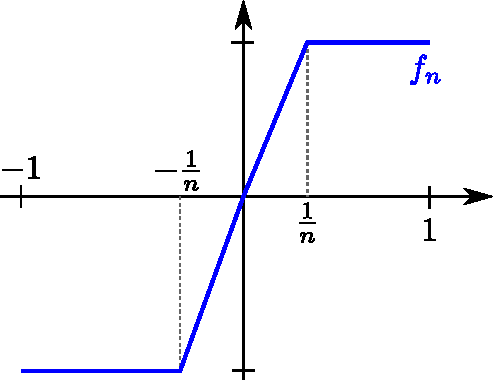
\includegraphics[width=.25\textwidth]{NichtvollstaendigkeitFolge.pdf}
	\vspace{-4em}\end{wrapfigure}
	
	Dazu haben wir für $n \in \NN$: die Funktion
		\[fn: [-1,1] \to \RR: x \mapsto \begin{cases}
			-1, &x \in [-1,-\frac{1}{n}] \\
			nx, &x \in ]-\frac{1}{n},\frac{1}{n}[ \\
			1,  &x \in [\frac{1}{n},1]
		\end{cases}\]
	definiert und gezeigt, dass $\left(f_n\right)$ eine Chauchy-Folge in $\mathcal{C}^0\left(\left[-1,1\right]\right)$ ist (also dass die $f_n$ stetige Funktionen sind und $\lInorm{f_n - f_m} \rightarrow 0$).
	
	Bleibt also noch zu zeigen, dass die Folge $(f_n)$ trotzdem nicht konvergiert. Das haben wir gemacht, indem wir annahmen, die Folge hätte einen Grenzwert $f \in \mathcal{C}^0\left(\left[-1,1\right]\right)$, und dies zu einem Widerspruch führen. Damit hatten wir gezeigt, dass die Folge keinen Grenzwert haben kann, und waren fertig.
	
	\vspace{1em}
	
	Soweit, so gut. Nun gibt es aber noch einen zweiten scheinbar einfacheren und vielleicht auch näherliegenden Lösungsweg:
	
	Wir finden einen Grenzwert $\tilde{f}$ und zeigen dann, dass dieser nicht in $\mathcal{C}^0\left(\left[-1,1\right]\right)$ liegt (also nicht stetig ist). Damit haben wir gezeigt, dass \emph{der} Grenzwert der Chauchy-Folge $(f_n)$ nicht in $\mathcal{C}^0\left(\left[-1,1\right]\right)$ liegt - folglich ist dieser Raum nicht vollständig.
	
	Dieser \glqq Beweis\grqq{} erscheint vor allem dann plausibel (zumindest mir), wenn man ihn anschaulich führt:
	
	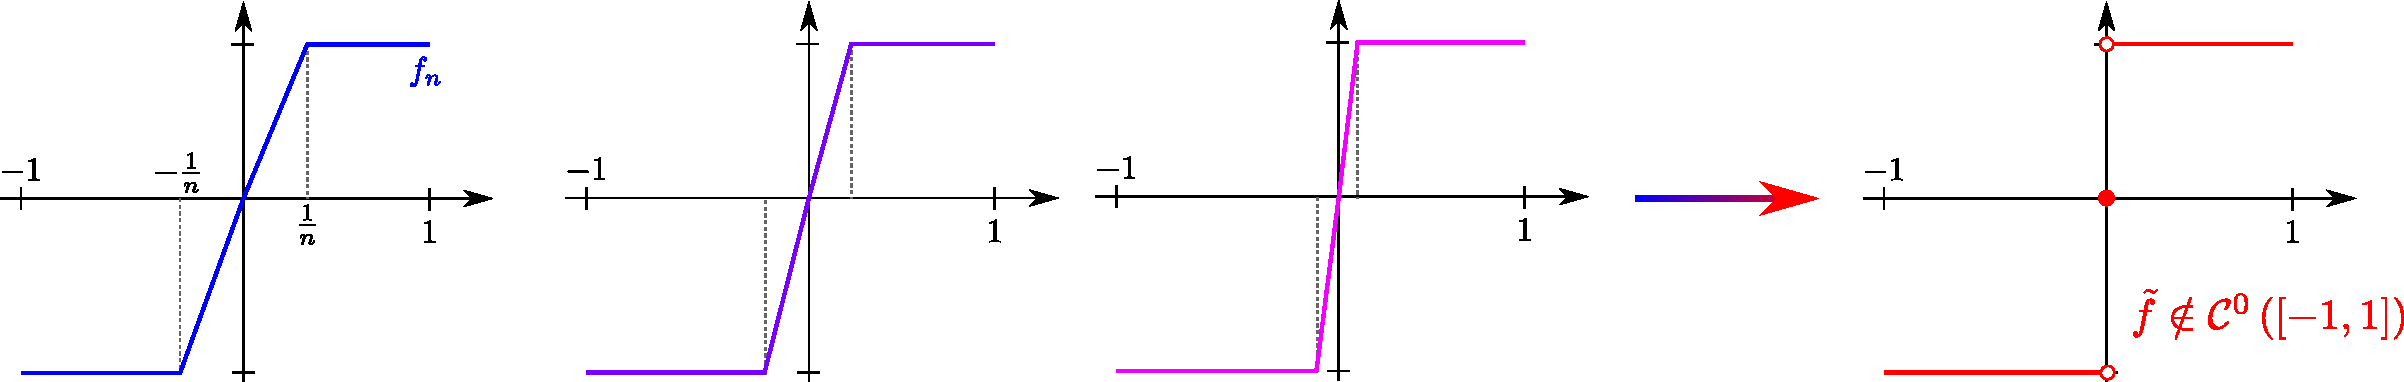
\includegraphics[width=\textwidth]{NichtvollstaendigkeitAnschaulicheKonvergenz.pdf}
	
	Der Grenzwert von $f_n$ ist \glqq offensichtlich\grqq{} die Funktion
		\[\tilde{f}: [-1,1] \to \RR: x \mapsto \begin{cases}
			-1, &x<0 \\
			0,  &x=0 \\
			1,  &x>0
		\end{cases}\]
	und diese ist offensichtlich nicht stetig.
	
	\newpage
	
	Dass an diesem \glqq Beweis\grqq{} etwas faul ist, habe ich euch mit folgendem Beispiel zu überzeugen versucht:
	
	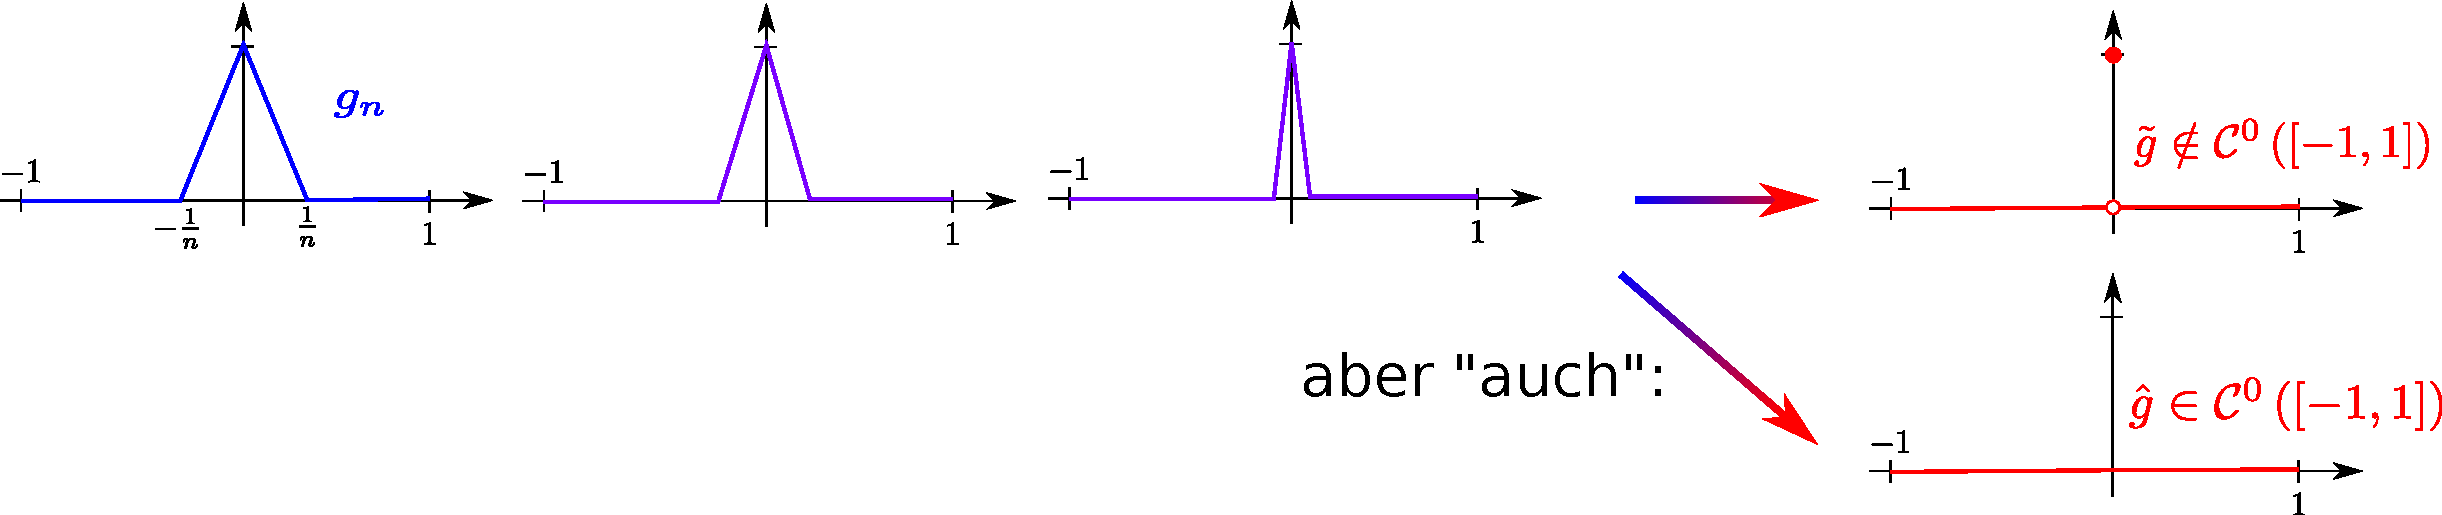
\includegraphics[width=\textwidth]{NichtvollstaendigkeitGegenbsp.pdf}
	
	Das zeigt zumindest schonmal, dass der obige \glqq Beweis\grqq{} in dieser Form nicht völlig in Ordnung sein kann. Es bleibt aber noch die Frage offen, was \emph{genau} in diesem schief gelaufen ist. Um das besser sehen (und hoffentlich verstehen) zu können, schreibe ich den \glqq Beweis\grqq{} jetzt nochmal formal auf:
	
	\begin{proof}
	Sei $\tilde{f}$ wie oben definiert. Dann gilt:
		\[\lInorm{f-f_n} = \int_{-1}^1\left|f(x)-f_n(x)\right|dx = \int_{-\frac{1}{n}}^{\frac{1}{n}}\left|f(x)-f_n(x)\right|dx \leq \int_{-\frac{1}{n}}^{\frac{1}{n}}2dx=\frac{4}{n}\to 0\]
	Also konvergiert $f_n$ gegen $\tilde{f} \notin \mathcal{C}^0\left(\left[-1,1\right]\right)$. Fertig!?
	
	Naja, noch nicht ganz: Wir haben gezeigt, dass unsere Folge \emph{einen} Grenzwert \emph{außerhalb} unseres Raumes hat. Zeigen müssen wir aber, dass die Folge \emph{keinen} Grenzwert \emph{innerhalb} unseres Raumes hat. Damit letzteres aus ersterem folgt, müssten wir noch wissen, dass Grenzwerte eindeutig sind (jede Folge also höchstens einen Grenzwert hat).
	
	In allgemeinen topologischen Räumen ist das \emph{falsch}, es wird aber richtig, sobald unser Raum hausdorffsch ist (warum? Einfache Übungsaufgabe...!). Und normierte Räume sind sicher hausdorffsch. Damit können wir unseren \glqq Beweis\grqq{} nun vervollständigen:
	
	Der \emph{eindeutige} (also insbesondere \emph{einzige}) Grenzwert von $f_n$ liegt nicht in $\mathcal{C}^0\left(\left[-1,1\right]\right)$. Folglich hat $f_n$ keinen Grenzwert in $\mathcal{C}^0\left(\left[-1,1\right]\right)$.
	\end{proof}
	
	Sieht doch eigentlich nach einen ganz guten Beweis aus, oder? Trotzdem behaupte ich, dass das so nicht stimmt (und unser Gegenbeispiel zeigt das ja auch). Was ist also schief gelaufen?
	
	Falls dir das nicht eh schon klar ist, empfehle ich sehr den obigen Beweis nochmal genau zu lesen, und nach möglichen Fehlerstellen zu suchen. Das ist nämlich eine hervorragende Übung (darum freue ich mich auch immer eure Übungsblätter korrigieren zu dürfen :-).
	
	Evtl. hilft es dabei den obigen Beispiel für das Gegenbeispiel umzuschreiben. Spätestens da muss dann ja etwas schief gehen...
	
	\newpage
	
	Was ist nun also schief gelaufen? Soweit ich das sehe, gibt es im wesentlichen zwei Stellen, an denen der \glqq Beweis\grqq{} fehlerhaft ist (wer weitere findet, bitte Bescheid sagen):
	
	\begin{enumerate}
		\item Was ist eigentlich $\lInorm{f-f_n}$? $\lInorm{.}$ ist doch eine Norm auf dem Raum der stetigen Funktionen ($\mathcal{C}^0\left(\left[-1,1\right]\right)$) - jetzt setzen wir aber plötzlich eine nicht-stetige Funktion darin ein (nämlich $f-f_n$). Das ist natürlich Quatsch!\footnote{Es ist ungefähr so als würde eine Schülerin, die gerade die Wurzelfunktion kennengelernt hat, plötzlich negative Zahlen in die Wurzelfunktion einsetzen.}
		
		Warum kommt oben dann trotzdem etwas \glqq sinnvolles\grqq{} heraus? Nun, wir haben - ohne das zu erwähnen - die Funktion $\lInorm{.}$ auf einen größeren Definitionsbereich ausgedehnt (etwa auf $\mathcal{R}\left(\left[-1,1\right]\right)$). Da dort die gleiche Funktionsvorschrift zufälligerweise immer noch zu einem sinnvollen Ergebnis führt, ist das nicht weiter aufgefallen.\footnote{Im Beispiel der Wurzelfunktion wäre das so, als hätte die Schülerin nun noch etwas über die komplexen Zahlen gehört. Denn dann kann sie die Wurzelfunktion auch auf negative Zahlen ausweiten (und verwirrenderweise für beide Funktionen das gleiche Symbol verwenden).}
		
		Das entscheidende Problem, das dabei unter den Tisch fällt, ist, dass die erweiterte Funktion nicht mehr zwangsläufig alle Eigenschaften der ursprünglichen Funktion hat. In unserem Falle geht es dabei insbesondere um die Eigenschaft eine Norm zu sein. Und tatsächlich ist $\lInorm{.}$ auf $\mathcal{R}\left(\left[-1,1\right]\right)$ \emph{keine} Norm mehr (sondern nur noch eine Halbnorm).\footnote{Auch im Wurzelbeispiel tritt dieses Problem auf: Die auf ganz $\RR$ erweiterte Wurzelfunktion behält ebenfalls nicht alle Eigenschaften der Wurzelfunktion auf $\RR_{\geq 0}$, wie die folgende Rechnung zeigt:
			\[1 = \sqrt{1} = \sqrt{(-1)(-1)} = \sqrt{-1}\sqrt{-1}=i\cdot i = -1\]
		Hier geht also die Multiplikativität der Wurzelfunktion verloren.}
	
		Ab diesem Punkt dürfen wir also nicht mehr einfach so annehmen, dass die Normaxiome für $\lInorm{.}$ erfüllt sind (und tatsächlich ist nun die Definiertheit nicht mehr erfüllt). Genau das tun wir aber - erneut ein wenig versteckt - im letzten Schritt. Was uns zum zweiten Problempunkt führt:
		
		\item Um am Ende sicherzustellen, dass der gefundene (nicht-stetige) Grenzwert auch schon der einzige mögliche Grenzwert ist, verwenden wir, dass \glqq unser Raum\grqq{} normiert (und damit hausdorffsch) ist. Was aber genau ist \glqq unser Raum\grqq{}?
		
		Ein naheliegender Gedanke wäre $\mathcal{C}^0\left(\left[-1,1\right]\right)$ - denn dieser ist versehen mit der Norm $\lInorm{.}$ auch wirklich normiert. Dummerweise liegt nun aber der Punkt, um den es hier geht - nämlich die Funktion $\tilde{f}$ - überhaupt nicht in diesem Raum.
		
		Wir müssen hier also einen anderen, größeren Raum betrachten, der auch $\tilde{f}$ miteinschließt. Beispielsweise $\mathcal{R}\left(\left[-1,1\right]\right)$. Dieser enthält sicher alle Funktionen, die wir hier betrachten - bezüglich der (erweiterten - s.o.) Abbildung $\lInorm{.}$ ist er aber kein normierter Raum mehr.
		
		Also ist dieser Raum nicht mehr zwangsläufig hausdorffsch (bzgl. der von der Halbnorm $\lInorm{.}$ induzierten Topologie) und wir wissen auch nicht mehr, dass Grenzwerte zwangsläufig eindeutig sind. Und tatsächlich gehen hier auch beide diese Eigenschaften schief: Wir können nämlich Funktionen in $\mathcal{R}\left(\left[-1,1\right]\right)$ nicht mehr voneinander unterscheiden, wenn sie nur an einzelnen Punkten unterschiedlich sind.
		
		Insbesondere kann eine Folge (von Funktionen!) in diesem Raum also problemlos mehrere Grenzwerte haben (nimm einen bestimmten Grenzwert (also eine Funktion), ändere die Funktion an einem einzelnen Punkt ab, und schon hast du einen neuen Grenzwert der Folge). Und wie das Gegenbeispiel zeigt, kann es durchaus passieren, dass manche der Grenzwerte nicht in $\mathcal{C}^0\left(\left[-1,1\right]\right)$ liegen - ein andere dann aber doch.
		
		Damit ist dann auch klar, dass es nicht genügt, zu zeigen, dass \emph{ein} Grenzwert nicht in $\mathcal{C}^0\left(\left[-1,1\right]\right)$ liegt. Sondern vielmehr müssen wir zeigen, dass \emph{jeder} Grenzwert nicht in $\mathcal{C}^0\left(\left[-1,1\right]\right)$ liegt.
	\end{enumerate}
	
	\hrulefill
	
	Da die Anschauung bei Funktionenräumen manchmal etwas schwer fällt, hätte ich zum Abschluss noch den Versuch eines analogen Beispiels in einem viel einfacheren Raum:
		
	Wir betrachten nämlich einfach $\RR$ (mit der Standardnorm $\vert.\vert_\RR$). Dieser ist, wie wir aus Analysis I wissen, vollständig. Ich werde nun aber beweisen, dass dieser nicht-vollständig ist (mit einem \glqq Beweis\grqq{} ganz analog zu dem oben):
	
	\begin{proof}
		Wir betrachten die Folge $\frac{1}{n}$ - diese ist sicher eine Chauchy-Folge, sollte also einen Konvergenzpunkt (in $\RR$) besitzen. Um zu zeigen, dass dem nicht so ist, betrachten wir den größeren Raum $\CC$. Und erweitern unsere Norm von $\RR$ wie folgt\footnote{die Abbildung, die wir durch diese Erweiterung erhalten, entspricht natürlich nicht der \glqq gewöhnlichen\grqq{} Norm von $\CC$. Schon allein deshalb weil sie - wie im Anfangsbeispiel - überhaupt keine Norm ist.}:
		\[\left\vert.\right\vert_\RR: \CC \to \RR: x+iy \mapsto \left\vert x \right\vert\]
		Damit ist nun aber $0+i \in \CC$ ein Grenzwert unserer Folge $\frac{1}{n}$, denn es gilt:
			\[\left\vert 0+i - \frac{1}{n}\right\vert_\RR = \left\vert i - \frac{1}{n}\right\vert_\RR = \left\vert\frac{1}{n}\right\vert \to 0\]
		Also ist der Grenzwert von $\frac{1}{n}$ die Zahl $i$, welche nicht in $\RR$ liegt - und unsere Folge hat daher keinen Grenzwert in $\RR$. Folglich ist $\RR$ nicht vollständig - ups...
	\end{proof}
	
	\begin{center}
		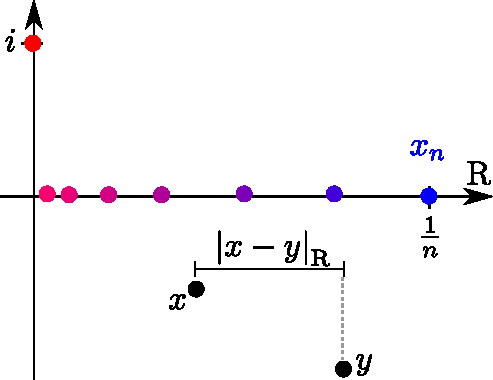
\includegraphics[width=.4\textwidth]{Nichtvollstaendigkeit2DAnalog.pdf}
	\end{center}
	
	Auch hier muss ich natürlich irgendwo geschummelt haben - und tatsächlich habe ich das genau an den gleichen Stellen (und auf die gleiche Weise) wie in obigem \glqq Beweis\grqq .	
	
	\begin{bem}
		Allgemein sollte man ein wenig vorsichtig sein, wenn man sich Probleme in unendlich dimensionalen Vektorräumen (wie $\mathcal{C}^0\left(\left[-1,1\right]\right)$) anhand von endlich dimensionalen (wie $\RR$) veranschaulicht. Beim Übergang von endlichen zu unendlichen Dimensionen, passieren nämlich einige durchaus wesentlichen Änderungen\footnote{weswegen man unendlich Dimensionale Vektorräume meistens auch erst in Linearer Algebra III (die aus irgendwelchen seltsamen Gründen Funktionalanalysis heißt) richtig kennenlernt. Dort lernt man dann auch wie man das Problem mit der Halbnorm wieder in den Griff bekommt (für die algebraisch interessierten: Das entscheidende Stichwort ist \glqq Quotientenraum\grqq ).} - ich glaube aber, dass in diesem Falle alle hier interessanten Punkte ausreichend gut erhalten bleiben.
	\end{bem}
	
	 
	
	
\end{document}